% =============================================================================
% SPARC — Presentation Slides (Research Storytelling Version)
% Style: Madrid (stripped) + Navy/White/Gold + TikZ + pgfplots + fontawesome
% =============================================================================
\documentclass[aspectratio=169, 11pt]{beamer}

% ---- Theme ----
\usetheme{Madrid}
\usecolortheme{default}

% ---- Packages ----
\usepackage{fontspec}
\usepackage{amsmath,amssymb}
\usepackage{tikz}
\usetikzlibrary{shapes,arrows.meta,positioning,calc,fit,backgrounds,decorations.pathreplacing}
\usepackage{pgfplots}
\pgfplotsset{compat=1.18}
\usepackage{fontawesome5}
\usepackage{booktabs}
\usepackage{colortbl}
\usepackage{graphicx}
\usepackage{hyperref}
\usepackage{multicol}

% ---- Color Palette: Navy / White / Gold ----
\definecolor{navydark}{HTML}{0D1B2A}
\definecolor{navymid}{HTML}{1B2838}
\definecolor{navyblue}{HTML}{1B3A5C}
\definecolor{steelblue}{HTML}{415A77}
\definecolor{lightslate}{HTML}{778DA9}
\definecolor{warnorange}{HTML}{E8943A}
\definecolor{goldaccent}{HTML}{F0C040}
\definecolor{successgreen}{HTML}{2ECC71}
\definecolor{dangerred}{HTML}{E74C3C}
\definecolor{softwhite}{HTML}{F0F4F8}

% ---- Override Beamer Colors ----
\setbeamercolor{structure}{fg=navyblue}
\setbeamercolor{palette primary}{bg=navydark,fg=white}
\setbeamercolor{palette secondary}{bg=navymid,fg=white}
\setbeamercolor{palette tertiary}{bg=navyblue,fg=white}
\setbeamercolor{palette quaternary}{bg=steelblue,fg=white}
\setbeamercolor{frametitle}{bg=navydark,fg=white}
\setbeamercolor{title}{fg=white}
\setbeamercolor{subtitle}{fg=goldaccent}
\setbeamercolor{author}{fg=softwhite}
\setbeamercolor{date}{fg=lightslate}
\setbeamercolor{item}{fg=warnorange}
\setbeamercolor{block title}{bg=navyblue,fg=white}
\setbeamercolor{block body}{bg=softwhite,fg=navydark}
\setbeamercolor{block title alerted}{bg=dangerred,fg=white}
\setbeamercolor{block body alerted}{bg=dangerred!10,fg=navydark}
\setbeamercolor{block title example}{bg=successgreen!80!black,fg=white}
\setbeamercolor{block body example}{bg=successgreen!10,fg=navydark}
\setbeamercolor{footline}{bg=navydark,fg=lightslate}
\setbeamercolor{navigation symbols}{fg=lightslate}

\setbeamerfont{title}{size=\Large,series=\bfseries}
\setbeamerfont{subtitle}{size=\normalsize}
\setbeamerfont{frametitle}{size=\large,series=\bfseries}

% ---- Metadata ----
\title{SPARC}
\subtitle{Lightweight Altitude-Aware Cross-View Geo-Localization}
\author{Tran Chi Nguyen$^*$ \quad Dao Sy Duy Minh$^*$ \quad Huynh Trung Kiet$^*$ \\ Pham Phu Hoa \quad Nguyen Lam Phu Quy}
\date{\today}

\begin{document}

% =========================================================================
% SLIDE 1: TITLE
% =========================================================================
{
\setbeamertemplate{footline}{}
\begin{frame}[plain]

\begin{tikzpicture}[remember picture,overlay]
  \fill[navydark] (current page.south west) rectangle (current page.north east);
  \fill[navymid,opacity=0.6] ([yshift=2cm]current page.south west) rectangle (current page.north east);
  \fill[navyblue,opacity=0.3] ([yshift=5cm]current page.south west) rectangle (current page.north east);

  \draw[warnorange, line width=2pt] ([xshift=1.5cm,yshift=4.8cm]current page.south west)
    -- ([xshift=14.5cm,yshift=4.8cm]current page.south west);

  \node[anchor=west,text=white,font=\huge\bfseries] at ([xshift=1.5cm,yshift=6.8cm]current page.south west)
    {SPARC: \normalsize Semantic Part-Aware Retrieval for Cross-view};

  \node[anchor=west,text=goldaccent,font=\large] at ([xshift=1.5cm,yshift=5.8cm]current page.south west)
    {Lightweight Altitude-Aware Cross-View Geo-Localization};

  \node[anchor=west,text=lightslate,font=\normalsize] at ([xshift=1.5cm,yshift=5.2cm]current page.south west)
    {Part Discovery $\cdot$ Multi-Level Distillation $\cdot$ Masked Reconstruction};

  \node[anchor=west,text=softwhite,font=\normalsize] at ([xshift=1.5cm,yshift=3.8cm]current page.south west)
    {\faUsers\ \ Tran Chi Nguyen$^*$ \quad Dao Sy Duy Minh$^*$ \quad Huynh Trung Kiet$^*$};

  \node[anchor=west,text=lightslate,font=\small] at ([xshift=1.5cm,yshift=3.2cm]current page.south west)
    {\phantom{\faUsers}\ \ Pham Phu Hoa \quad Nguyen Lam Phu Quy};

  \node[anchor=west,text=lightslate,font=\small] at ([xshift=1.5cm,yshift=2.6cm]current page.south west)
    {\faCalendar\ \ \today};
\end{tikzpicture}
\end{frame}
}

% =========================================================================
% SLIDE 2: OUTLINE
% =========================================================================
\begin{frame}{Outline}
\centering
\vspace{0.1cm}
\begin{tikzpicture}[
  num/.style={circle, fill=navyblue, text=white, font=\bfseries, minimum size=0.6cm, inner sep=0pt},
  item/.style={font=\normalsize, text=navydark, anchor=west},
  icon/.style={font=\small, text=warnorange, anchor=west},
]
  \node[num] (n1) at (0, 3.6) {1};
  \node[icon] at (0.6, 3.6) {\faCrosshairs};
  \node[item] at (1.1, 3.6) {Motivation \& Problem};

  \node[num] (n2) at (0, 2.7) {2};
  \node[icon] at (0.6, 2.7) {\faHistory};
  \node[item] at (1.1, 2.7) {Evolution of Methods};

  \node[num] (n3) at (0, 1.8) {3};
  \node[icon] at (0.6, 1.8) {\faExclamationTriangle};
  \node[item] at (1.1, 1.8) {Limitations of Prior Work};

  \node[num] (n4) at (0, 0.9) {4};
  \node[icon] at (0.6, 0.9) {\faGraduationCap};
  \node[item] at (1.1, 0.9) {Our Method};

  \node[num] (n5) at (0, 0.0) {5};
  \node[icon] at (0.6, 0.0) {\faProjectDiagram};
  \node[item] at (1.1, 0.0) {\textbf{Core Novelty: Semantic Part Graph}};

  \node[num] (n6) at (0, -0.9) {6};
  \node[icon] at (0.6, -0.9) {\faCogs};
  \node[item] at (1.1, -0.9) {Multi-Task Training \& Self-Supervision};

  \node[num] (n7) at (0, -1.8) {7};
  \node[icon] at (0.6, -1.8) {\faTrophy};
  \node[item] at (1.1, -1.8) {Results, Ablation \& Final Positioning};

  \begin{scope}[on background layer]
    \draw[navyblue!20, line width=2pt] (n1.south) -- (n7.north);
  \end{scope}
\end{tikzpicture}
\end{frame}

% =========================================================================
% SLIDE 3: MOTIVATION
% =========================================================================
\begin{frame}{Motivation: Why Cross-View Geo-Localization?}
\begin{columns}[T]
\column{0.52\textwidth}
\vspace{0.2cm}
{\large \textbf{\faCrosshairs\ \ The Problem}}
\vspace{0.2cm}

\begin{itemize}
  \setlength\itemsep{0.6em}
  \item \textbf{Goal:} Given a drone query $\rightarrow$ retrieve matching satellite image from a large gallery
  \item \textbf{Core challenge:} Extreme viewpoint gap between oblique drone and top-down satellite views
  \item \textbf{Altitude variation:} Low altitude captures local detail;high altitude reveals global layout
\end{itemize}

\column{0.44\textwidth}
\vspace{0.2cm}
\begin{exampleblock}{\faLightbulb\ \ The Question}
  \itshape How do you localize a drone when GPS fails?\\
  Match what it sees to a satellite map ---\\
  but the viewpoint gap is extreme.
\end{exampleblock}

\vspace{0.3cm}
{\large \textbf{\faExclamation\ \ Why It's Hard}}
\vspace{0.1cm}
\begin{itemize}
  \item Viewpoint: oblique vs.\ top-down
  \item Scale: altitude changes field of view
  \item Appearance: lighting, season, occlusion
\end{itemize}
\end{columns}
\end{frame}

% =========================================================================
% SLIDE 4: EVOLUTION OF METHODS
% =========================================================================
\begin{frame}{Evolution of Cross-View Geo-Localization}
\footnotesize
\centering
\begin{tabular}{@{}l l c c l l@{}}
  \toprule
  \textbf{Era} & \textbf{Method} & \textbf{Backbone} & \textbf{Params} & \textbf{Strength} & \textbf{Weakness} \\
  \midrule
  2022 & LPN & ResNet-50 & $\sim$49M & Simple, fast & Weak alignment \\
  2022 & FSRA & ViT-S & $\sim$52M & Feature square & Heavy \\
  2023 & DWDR & ResNet-152 & $\sim$60M & Graph / geometry & Slow inference \\
  2023 & Sample4Geo & ConvNeXt-B & $\sim$88M & Hard-neg sampling & 4$\times$ heavier \\
  2023 & MCCG & ConvNeXt-B & $\sim$91M & Multi-classifier & No altitude cond. \\
  2024 & CAMP & ConvNeXt-B & $\sim$91M & Cross-attn map & Heavy backbone \\
  2024 & SeGCN & ConvNeXt & $\sim$28M & Graph conv & No distillation \\
  2025 & MCFA & ConvNeXt & $\sim$28M & Multi-scale fusion & Multi-stage \\
  2025 & GLQINet & ConvNeXt & $\sim$28M & Quadrant interaction & No distillation \\
  \midrule
  \rowcolor{successgreen!15}
  2026 & \textbf{SPARC (Ours)} & \textbf{DINOv2 ViT-S} & \textbf{$\sim$22M} & \textbf{Semantic parts + SOTA} & \textbf{---} \\
  \bottomrule
\end{tabular}
\end{frame}

% =========================================================================
% SLIDE 5: LIMITATIONS OF PRIOR WORK
% =========================================================================
\begin{frame}{Limitations of Prior Work}
\begin{columns}[T]
\column{0.32\textwidth}
\centering

\begin{tikzpicture}
  \node[circle, fill=dangerred!15, minimum size=2cm, draw=dangerred!50, line width=1pt] (c1)
    {\Large \faServer};
  \node[below=0.2cm of c1, font=\small\bfseries, text=navydark] {Heavy Models};
\end{tikzpicture}
\vspace{0.2cm}
\begin{itemize}\footnotesize
  \item ViT-B/16 at 86M params
  \item Impractical for edge/UAV
  \item Slow inference ($>$50ms)
\end{itemize}

\column{0.32\textwidth}
\centering

\begin{tikzpicture}
  \node[circle, fill=warnorange!15, minimum size=2cm, draw=warnorange!50, line width=1pt] (c2)
    {\Large \faCubes};
  \node[below=0.2cm of c2, font=\small\bfseries, text=navydark] {Limited Structure};
\end{tikzpicture}
\vspace{0.2cm}
\begin{itemize}\footnotesize
  \item Most methods rely on global descriptors
  \item Semantic part relations underexplored
  \item Limited viewpoint-invariant reasoning
\end{itemize}

\column{0.32\textwidth}
\centering

\begin{tikzpicture}
  \node[circle, fill=navyblue!15, minimum size=2cm, draw=navyblue!50, line width=1pt] (c3)
    {\Large \faChartArea};
  \node[below=0.2cm of c3, font=\small\bfseries, text=navydark] {Altitude-Blind};
\end{tikzpicture}
\vspace{0.2cm}
\begin{itemize}\footnotesize
  \item Ignore altitude variation
  \item 150m $\neq$ 300m image
  \item No altitude conditioning
\end{itemize}
\end{columns}

\vspace{0.4cm}
\centering
\begin{tikzpicture}
  \node[fill=goldaccent!15, rounded corners=6pt, inner sep=8pt, draw=goldaccent!50, font=\small, text=navydark] {
    \faArrowRight\ \ \textbf{These gaps motivate:} lightweight distillation + part reasoning + altitude awareness
  };
\end{tikzpicture}
\end{frame}

% =========================================================================
% SLIDE 6: WHY DISTILLATION + OUR METHOD
% =========================================================================
\begin{frame}{Why Distillation + Our Approach}
\begin{columns}[T]
\column{0.48\textwidth}
\vspace{0.2cm}
{\large \textbf{\faGraduationCap\ \ Why Distillation?}}
\vspace{0.2cm}
\begin{itemize}
  \setlength\itemsep{0.6em}
  \item Teacher $\rightarrow$ student works for CVGL
  \item CNN student limits spatial reasoning
  \item \textbf{Our choice:} DINOv2 ViT-S/14, 22M params
\end{itemize}

\column{0.48\textwidth}
\vspace{0.2cm}
{\large \textbf{\faLightbulb\ \ Our Key Insight}}
\vspace{0.2cm}

\begin{exampleblock}{Beyond feature mimicry}
  Discover \textbf{semantic parts} of the scene.\\[0.2em]
  Parts = \textbf{implicit spatial graph}.\\[0.2em]
  Condition on \textbf{flight altitude}.
\end{exampleblock}
\end{columns}
\end{frame}

% =========================================================================
% SLIDE 6b: WHY PRIOR GRAPH APPROACHES FAIL
% =========================================================================
\begin{frame}{Why Prior Graph Approaches Fail}
\centering
\vspace{-0.1cm}

\begin{tikzpicture}[
  nd/.style={circle, fill=#1, minimum size=6pt, inner sep=0pt, draw=#1!70!black, line width=0.5pt},
  lbl/.style={font=\scriptsize, text=navydark},
  boxx/.style={rectangle, rounded corners=4pt, draw=#1, fill=#1!5, minimum width=4.2cm, minimum height=5.2cm, inner sep=6pt},
]
  % === (a) Handcrafted Graph ===
  \node[boxx=dangerred] at (0, 0) {};
  \node[font=\small\bfseries, text=dangerred] at (0, 2.2) {(a) Handcrafted Graph};
  \node[font=\scriptsize\itshape, text=lightslate] at (0, 1.75) {Fixed class-to-class edges};

  % nodes
  \node[nd=steelblue] (a1) at (-0.9, 1.1) {};
  \node[font=\tiny, text=steelblue, above=1pt of a1] {car};
  \node[nd=successgreen!80!black] (a2) at (0.0, 1.2) {};
  \node[font=\tiny, text=successgreen!80!black, above=1pt of a2] {road};
  \node[nd=warnorange] (a3) at (0.9, 1.1) {};
  \node[font=\tiny, text=warnorange, above=1pt of a3] {tree};
  \node[nd=lightslate] (a4) at (-0.5, 0.4) {};
  \node[font=\tiny, text=lightslate, below=1pt of a4] {sky};
  \node[nd=dangerred!70] (a5) at (0.7, 0.3) {};
  \node[font=\tiny, text=dangerred!70, below=1pt of a5] {goat};
  % fixed edges (some missing)
  \draw[thick, steelblue!50] (a1) -- (a2);
  \draw[thick, successgreen!50] (a2) -- (a3);
  \draw[thick, lightslate!50] (a1) -- (a4);
  % goat is alone - isolated!
  \node[font=\tiny\itshape, text=dangerred, anchor=west] at (0.95, 0.0) {\faQuestion\ alone};
  % text
  \node[lbl, text width=3.8cm, align=center] at (0, -0.8) {
    \textcolor{dangerred}{\faTimesCircle}\ Cannot adapt to context\\[1pt]
    \textcolor{dangerred}{\faTimesCircle}\ Linguistic $\neq$ visual\\[1pt]
    \textcolor{dangerred}{\faTimesCircle}\ Relations ignored
  };

  % === (b) Fully Connected ===
  \node[boxx=warnorange] at (5.2, 0) {};
  \node[font=\small\bfseries, text=warnorange] at (5.2, 2.2) {(b) Fully Connected};
  \node[font=\scriptsize\itshape, text=lightslate] at (5.2, 1.75) {All-to-all edges};

  % nodes
  \node[nd=steelblue] (b1) at (4.3, 1.1) {};
  \node[nd=successgreen!80!black] (b2) at (5.2, 1.3) {};
  \node[nd=warnorange] (b3) at (6.1, 1.1) {};
  \node[nd=lightslate] (b4) at (4.6, 0.4) {};
  \node[nd=dangerred!70] (b5) at (5.8, 0.4) {};
  % ALL edges - messy
  \draw[thin, lightslate!40] (b1) -- (b2);
  \draw[thin, lightslate!40] (b1) -- (b3);
  \draw[thin, lightslate!40] (b1) -- (b4);
  \draw[thin, lightslate!40] (b1) -- (b5);
  \draw[thin, lightslate!40] (b2) -- (b3);
  \draw[thin, lightslate!40] (b2) -- (b4);
  \draw[thin, lightslate!40] (b2) -- (b5);
  \draw[thin, lightslate!40] (b3) -- (b4);
  \draw[thin, lightslate!40] (b3) -- (b5);
  \draw[thin, lightslate!40] (b4) -- (b5);
  % text
  \node[lbl, text width=3.8cm, align=center] at (5.2, -0.8) {
    \textcolor{dangerred}{\faTimesCircle}\ Redundant edges\\[1pt]
    \textcolor{dangerred}{\faTimesCircle}\ Background noise\\[1pt]
    \textcolor{dangerred}{\faTimesCircle}\ Signal $\ll$ noise
  };

  % === (c) Ours: Implicit Sparse ===
  \node[boxx=successgreen] at (10.4, 0) {};
  \node[font=\small\bfseries, text=successgreen!80!black] at (10.4, 2.2) {(c) Ours: Implicit \faStar};
  \node[font=\scriptsize\itshape, text=lightslate] at (10.4, 1.75) {Attention-driven sparse};

  % semantic part nodes
  \node[nd=warnorange, minimum size=8pt] (c1) at (9.5, 1.2) {};
  \node[font=\tiny, text=warnorange, above=1pt of c1] {Bldg};
  \node[nd=successgreen!80!black, minimum size=8pt] (c2) at (10.4, 0.7) {};
  \node[font=\tiny, text=successgreen!80!black, below=1pt of c2] {Road};
  \node[nd=warnorange, minimum size=8pt] (c3) at (11.3, 1.2) {};
  \node[font=\tiny, text=warnorange, above=1pt of c3] {Bldg};
  \node[nd=steelblue, minimum size=8pt] (c4) at (9.7, 0.2) {};
  \node[font=\tiny, text=steelblue, below=1pt of c4] {Veg};
  \node[nd=navyblue, minimum size=8pt] (c5) at (11.1, 0.2) {};
  \node[font=\tiny, text=navyblue, below=1pt of c5] {Water};
  % sparse meaningful edges only
  \draw[thick, successgreen!70!black] (c1) -- (c2);
  \draw[thick, successgreen!70!black] (c2) -- (c3);
  \draw[thick, steelblue!70] (c1) -- (c4);
  \draw[thick, navyblue!60] (c3) -- (c5);
  % text
  \node[lbl, text width=3.8cm, align=center] at (10.4, -0.8) {
    \textcolor{successgreen!80!black}{\faCheckCircle}\ Sparse \& adaptive\\[1pt]
    \textcolor{successgreen!80!black}{\faCheckCircle}\ Data-driven edges\\[1pt]
    \textcolor{successgreen!80!black}{\faCheckCircle}\ Viewpoint-invariant
  };

  % flow arrows
  \draw[->, >=stealth, thick, lightslate] (2.3, 0.7) -- node[above, font=\tiny, text=lightslate] {learn} (3.0, 0.7);
  \draw[->, >=stealth, thick, lightslate] (7.5, 0.7) -- node[above, font=\tiny, text=lightslate] {prune} (8.2, 0.7);
\end{tikzpicture}

\vspace{0.15cm}
\begin{tikzpicture}
  \node[fill=successgreen!15, rounded corners=6pt, inner sep=8pt, draw=successgreen!50, font=\small, text=navydark] {
    \faArrowRight\ \ Implicit part graph: \textbf{adapts to context}, \textbf{no redundant edges}, \textbf{viewpoint-invariant}
  };
\end{tikzpicture}
\end{frame}

% =========================================================================
% SLIDE 7: CORE NOVELTY — SEMANTIC PART GRAPH
% =========================================================================
\begin{frame}[fragile]{Core Novelty: Semantic Part Discovery}
\begin{columns}[T]
\column{0.48\textwidth}
\vspace{0.1cm}
{\large \textbf{\faProjectDiagram\ \ Semantic Parts (K=8)}}
\vspace{0.2cm}
\begin{itemize}
  \setlength\itemsep{0.5em}
  \item Learnable prototypes attend to DINOv2 patches
  \item Each part captures a semantic concept
  \item Parts + positions = \textbf{implicit scene graph}
  \item Structural relations are \textbf{viewpoint-invariant}
\end{itemize}

\vspace{0.2cm}
\begin{alertblock}{\faStar\ \ Novelty}
  \small \textbf{First} lightweight semantic part-level implicit graph formulation for CVGL.
\end{alertblock}

\column{0.48\textwidth}
\centering
\vspace{-0.2cm}
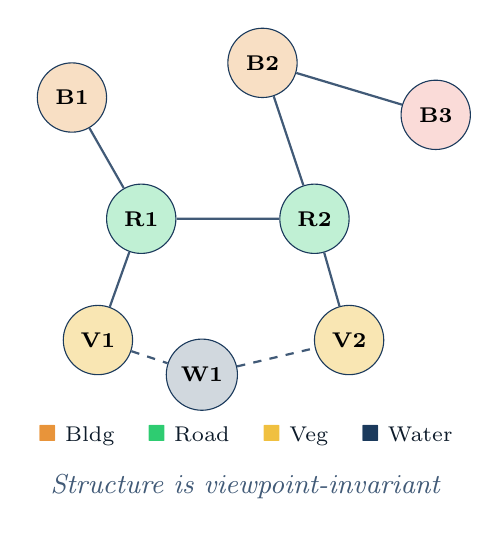
\begin{tikzpicture}[scale=1.1, transform shape,
  part/.style={circle, draw=navyblue, fill=#1, minimum size=0.8cm, font=\scriptsize\bfseries},
  edge/.style={thick, steelblue}]
  \node[part=warnorange!30] (b1) at (0,3.2) {B1};
  \node[part=warnorange!30] (b2) at (2.2,3.6) {B2};
  \node[part=successgreen!30] (r1) at (0.8,1.8) {R1};
  \node[part=successgreen!30] (r2) at (2.8,1.8) {R2};
  \node[part=goldaccent!40] (v1) at (0.3,0.4) {V1};
  \node[part=goldaccent!40] (v2) at (3.2,0.4) {V2};
  \node[part=navyblue!20] (w1) at (1.5,0) {W1};
  \node[part=dangerred!20] (b3) at (4.2,3) {B3};
  \draw[edge] (b1) -- (r1);  \draw[edge] (b2) -- (r2);
  \draw[edge] (r1) -- (r2);  \draw[edge] (r1) -- (v1);
  \draw[edge] (r2) -- (v2);  \draw[edge] (b2) -- (b3);
  \draw[edge, dashed] (v1) -- (w1); \draw[edge, dashed] (w1) -- (v2);
  \node[font=\scriptsize, text=navydark] at (2, -0.7) {
    \textcolor{warnorange}{$\blacksquare$} Bldg \quad
    \textcolor{successgreen}{$\blacksquare$} Road \quad
    \textcolor{goldaccent}{$\blacksquare$} Veg \quad
    \textcolor{navyblue}{$\blacksquare$} Water};
  \node[font=\small\itshape, text=steelblue] at (2, -1.3) {Structure is viewpoint-invariant};
\end{tikzpicture}
\end{columns}
\end{frame}

% =========================================================================
% SLIDE 8: ARCHITECTURE OVERVIEW
% =========================================================================
\begin{frame}{SPARC: Architecture Overview}
\centering
\vspace{-0.2cm}
\includegraphics[width=\textwidth, height=0.85\textheight, keepaspectratio]{architecture_infographic.png}
\end{frame}
% =========================================================================
% SLIDE 8b: WHY PROXY-BASED METRIC LEARNING
% =========================================================================
\begin{frame}{Why Proxy-Based Metric Learning?}
\centering
\vspace{-0.1cm}

% --- Row 1: Three TikZ visual diagrams ---
\begin{tikzpicture}[
  dot/.style={circle, fill=#1, minimum size=4pt, inner sep=0pt},
  proxy/.style={regular polygon, regular polygon sides=5, fill=#1, minimum size=8pt, inner sep=0pt, draw=#1!60!black},
  lbl/.style={font=\scriptsize, text=navydark},
  arr/.style={->, >=stealth, thin, #1},
  boxx/.style={rectangle, rounded corners=4pt, draw=#1, fill=#1!5, minimum width=4.2cm, minimum height=5.2cm, inner sep=6pt},
]
  % (a) Pair-Based
  \node[boxx=dangerred] (box1) at (0, 0) {};
  \node[font=\small\bfseries, text=dangerred] at (0, 2.2) {(a) Pair-Based};
  \node[font=\scriptsize\itshape, text=lightslate] at (0, 1.7) {Data $\leftrightarrow$ Data};
  % dots
  \foreach \x/\y/\c in {-0.8/0.8/steelblue, -0.3/1.1/steelblue, 0.3/0.6/dangerred, 0.8/1.0/dangerred, -0.5/0.2/successgreen!80!black, 0.6/0.3/successgreen!80!black} {
    \node[dot=\c] at (\x, \y) {};
  }
  % arrows between pairs
  \draw[arr=steelblue!50, dashed] (-0.8,0.8) -- (-0.3,1.1);
  \draw[arr=dangerred!50, dashed] (0.3,0.6) -- (0.8,1.0);
  \draw[arr=lightslate, dashed] (-0.8,0.8) -- (0.3,0.6);
  \draw[arr=lightslate, dashed] (-0.3,1.1) -- (0.8,1.0);
  \draw[arr=lightslate, dashed] (-0.5,0.2) -- (0.6,0.3);
  \draw[arr=lightslate, dashed] (-0.8,0.8) -- (0.6,0.3);
  % text
  \node[lbl, text width=3.8cm, align=center] at (0, -0.7) {
    $O(N^2)$ pairs\\[2pt]
    \textcolor{dangerred}{\faTimesCircle}\ Slow sampling\\
    \textcolor{dangerred}{\faTimesCircle}\ Overfit on hard pairs
  };

  % (b) Proxy-Based
  \node[boxx=warnorange] (box2) at (5.2, 0) {};
  \node[font=\small\bfseries, text=warnorange] at (5.2, 2.2) {(b) Proxy-Based};
  \node[font=\scriptsize\itshape, text=lightslate] at (5.2, 1.7) {Data $\leftrightarrow$ Proxy};
  % proxies
  \node[proxy=steelblue] (pa) at (4.7, 0.9) {};
  \node[proxy=dangerred] (pb) at (5.7, 0.9) {};
  % dots around proxies
  \node[dot=steelblue] (d1) at (4.3, 0.5) {};
  \node[dot=steelblue] (d2) at (4.5, 1.3) {};
  \node[dot=steelblue] (d3) at (5.0, 0.4) {};
  \node[dot=dangerred] (d4) at (5.5, 0.4) {};
  \node[dot=dangerred] (d5) at (5.9, 1.3) {};
  \node[dot=dangerred] (d6) at (6.1, 0.5) {};
  % arrows to proxy only
  \draw[arr=steelblue!60] (d1) -- (pa);
  \draw[arr=steelblue!60] (d2) -- (pa);
  \draw[arr=steelblue!60] (d3) -- (pa);
  \draw[arr=dangerred!60] (d4) -- (pb);
  \draw[arr=dangerred!60] (d5) -- (pb);
  \draw[arr=dangerred!60] (d6) -- (pb);
  % text
  \node[lbl, text width=3.8cm, align=center] at (5.2, -0.7) {
    $O(N {\cdot} C)$ only\\[2pt]
    \textcolor{successgreen!80!black}{\faCheckCircle}\ Fast convergence\\
    \textcolor{dangerred}{\faTimesCircle}\ Lacks data-data info
  };

  % (c) Proxy-Anchor
  \node[boxx=successgreen] (box3) at (10.4, 0) {};
  \node[font=\small\bfseries, text=successgreen!80!black] at (10.4, 2.2) {(c) Proxy-Anchor \faStar};
  \node[font=\scriptsize\itshape, text=lightslate] at (10.4, 1.7) {Best of Both};
  % proxy anchor in center
  \node[proxy=successgreen!80!black, minimum size=10pt] (pc) at (10.4, 0.8) {};
  \node[font=\tiny, text=successgreen!80!black] at (10.4, 0.45) {\faAnchor};
  % data orbiting
  \node[dot=steelblue] (e1) at (9.6, 0.5) {};
  \node[dot=steelblue] (e2) at (9.8, 1.2) {};
  \node[dot=steelblue] (e3) at (10.0, 0.3) {};
  \node[dot=dangerred] (e4) at (10.8, 0.3) {};
  \node[dot=dangerred] (e5) at (11.0, 1.2) {};
  \node[dot=dangerred] (e6) at (11.2, 0.5) {};
  % arrows: both to proxy AND between data
  \draw[arr=successgreen!60!black] (e1) -- (pc);
  \draw[arr=successgreen!60!black] (e2) -- (pc);
  \draw[arr=successgreen!60!black] (e3) -- (pc);
  \draw[arr=successgreen!60!black] (e4) -- (pc);
  \draw[arr=successgreen!60!black] (e5) -- (pc);
  \draw[arr=successgreen!60!black] (e6) -- (pc);
  \draw[arr=steelblue!30, dashed] (e1) -- (e2);
  \draw[arr=dangerred!30, dashed] (e5) -- (e6);
  % text
  \node[lbl, text width=3.8cm, align=center] at (10.4, -0.7) {
    Rich grads + efficient\\[2pt]
    \textcolor{successgreen!80!black}{\faCheckCircle}\ All pos/neg per batch\\
    \textcolor{successgreen!80!black}{\faCheckCircle}\ + UAPA uncertainty
  };

  % flow arrows between boxes
  \draw[->, >=stealth, thick, lightslate] (2.3, 0.7) -- node[above, font=\tiny, text=lightslate] {faster} (3.0, 0.7);
  \draw[->, >=stealth, thick, lightslate] (7.5, 0.7) -- node[above, font=\tiny, text=lightslate] {richer} (8.2, 0.7);
\end{tikzpicture}

\vspace{0.2cm}
\begin{tikzpicture}
  \node[fill=successgreen!15, rounded corners=6pt, inner sep=8pt, draw=successgreen!50, font=\small, text=navydark] {
    \faArrowRight\ \ \textbf{First} proxy-based metric learning in CVGL --- combines rich gradients with efficient convergence
  };
\end{tikzpicture}
\end{frame}

% =========================================================================
% SLIDE 9: MULTI-TASK TRAINING
% =========================================================================
\begin{frame}[fragile]{Multi-Task Training}
\centering
\vspace{0.2cm}
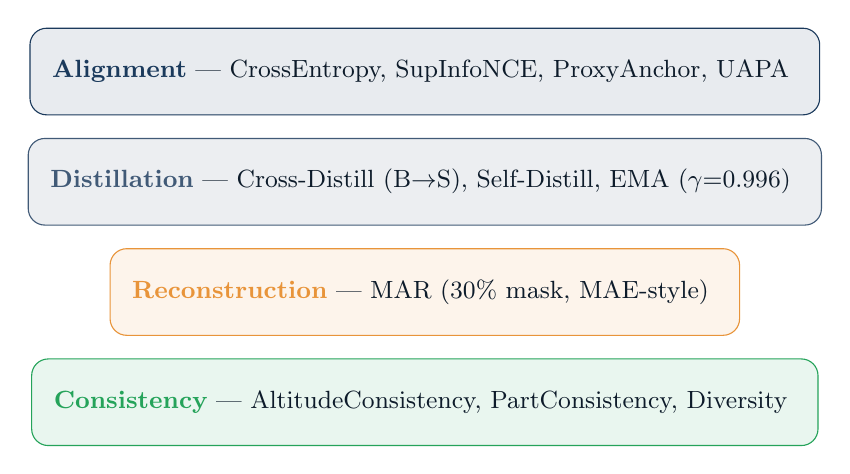
\begin{tikzpicture}[
  grp/.style={rectangle, rounded corners=6pt, draw=#1, fill=#1!10, minimum width=6cm,
              minimum height=1.1cm, font=\small, text=navydark, align=left, inner sep=8pt},
  lbl/.style={font=\small\bfseries, text=#1, anchor=west},
]
  \node[grp=navyblue] (a) at (0, 2.8) {
    \textbf{\textcolor{navyblue}{Alignment}} --- CrossEntropy, SupInfoNCE, ProxyAnchor, UAPA
  };
  \node[grp=steelblue] (d) at (0, 1.4) {
    \textbf{\textcolor{steelblue}{Distillation}} --- Cross-Distill (B$\to$S), Self-Distill, EMA ($\gamma$=0.996)
  };
  \node[grp=warnorange] (r) at (0, 0.0) {
    \textbf{\textcolor{warnorange}{Reconstruction}} --- MAR (30\% mask, MAE-style)
  };
  \node[grp=successgreen!80!black] (c) at (0, -1.4) {
    \textbf{\textcolor{successgreen!80!black}{Consistency}} --- AltitudeConsistency, PartConsistency, Diversity
  };
\end{tikzpicture}

\end{frame}

% =========================================================================
% SLIDE 9b: KEY COMPONENTS DETAIL
% =========================================================================
\begin{frame}{Key Components in Detail}
\begin{columns}[T]
\column{0.48\textwidth}
\vspace{0.1cm}
{\large \textbf{\faCogs\ \ Core Modules}}
\vspace{0.2cm}
\footnotesize
\begin{description}
  \setlength\itemsep{0.5em}
  \item[\textcolor{dangerred}{ProxyAnchor}] Proxy-based metric learning; assigns each class a learnable proxy for efficient hard-sample mining.
  \item[\textcolor{warnorange}{FusionGate}] Learned gating between CLS (global) and Part (local) descriptors:
    $f = \sigma(g) \cdot f_{\text{cls}} + (1{-}\sigma(g)) \cdot f_{\text{part}}$.
  \item[\textcolor{navyblue}{UAPA}] Uncertainty-Aware Proxy Anchor --- re-weights hard proxies via learned uncertainty.
\end{description}

\column{0.48\textwidth}
\vspace{0.1cm}
{\large \textbf{\faChartArea\ \ Altitude \& Consistency}}
\vspace{0.2cm}
\footnotesize
\begin{description}
  \setlength\itemsep{0.5em}
  \item[\textcolor{steelblue}{AltPred}] Auxiliary altitude prediction head on the Part branch; provides explicit altitude supervision.
  \item[\textcolor{lightslate}{DeepAltFiLM}] FiLM modulation conditioned on altitude --- scales and shifts intermediate features.
  \item[\textcolor{successgreen!80!black}{AltConsist}] Same-location embeddings across altitudes must be similar.
  \item[\textcolor{successgreen!80!black}{PartConsist}] Part prototypes stay stable across augmented views.
\end{description}
\end{columns}
\end{frame}

% =========================================================================
% SLIDE 10: MASKED PART RECONSTRUCTION
% =========================================================================
\begin{frame}{Self-Supervision: Masked Part Reconstruction}
\begin{columns}[T]
\column{0.50\textwidth}
\vspace{0.2cm}
{\large \textbf{\faCube\ \ Why MAR?}}
\vspace{0.2cm}
\begin{itemize}
  \setlength\itemsep{0.5em}
  \item MAE (Masked Autoencoder) is widely used in NLP \& vision
  \item Traditional self-supervision uses augmentation only --- no \textbf{structural reasoning}
  \item MAR forces part prototypes to encode \textbf{complete spatial layout}, not just discriminative shortcuts
  \item In map-matching: parts must ``understand'' the \textbf{whole scene} even with occlusion/partial views
\end{itemize}

\vspace{0.2cm}
\begin{exampleblock}{\faLightbulb\ \ Novelty}
  \small \textbf{First} masked reconstruction on \textbf{semantic part prototypes} for cross-view retrieval.
\end{exampleblock}

\column{0.46\textwidth}
\vspace{0.1cm}
\centering
% Visual: mask → parts → reconstruct pipeline
\begin{tikzpicture}
  \node[rectangle, rounded corners=3pt, draw=steelblue, fill=steelblue!10,
        minimum width=2.8cm, minimum height=0.8cm, font=\scriptsize, text=navydark, align=center]
    (input) at (0, 3.8) {\faImage\ \ Image Patches};

  \node[rectangle, rounded corners=3pt, draw=dangerred, fill=dangerred!10,
        minimum width=2.8cm, minimum height=0.8cm, font=\scriptsize, text=navydark, align=center]
    (mask) at (0, 2.6) {\faMask\ \ Mask 30\%};

  \node[rectangle, rounded corners=3pt, draw=warnorange, fill=warnorange!10,
        minimum width=2.8cm, minimum height=0.9cm, font=\scriptsize, text=navydark, align=center]
    (parts) at (0, 1.35) {\faCubes\ \ Part Prototypes};

  \node[rectangle, rounded corners=3pt, draw=successgreen!80!black, fill=successgreen!10,
        minimum width=2.8cm, minimum height=0.9cm, font=\scriptsize, text=navydark, align=center]
    (recon) at (0, 0.1) {\faMagic\ \ Reconstruct};

  \draw[->, >=stealth, thick, steelblue!70] (input) -- (mask);
  \draw[->, >=stealth, thick, dangerred!70] (mask) -- (parts);
  \draw[->, >=stealth, thick, warnorange!70] (parts) -- (recon);

  % side annotations
  \node[font=\tiny\itshape, text=lightslate, anchor=west, text width=1.5cm] at (1.6, 1.35) {Attend to visible patches};
  \node[font=\tiny\itshape, text=lightslate, anchor=west, text width=1.5cm] at (1.6, 2.6) {Epoch 10+};
  \node[font=\tiny\itshape, text=lightslate, anchor=west, text width=1.5cm] at (1.6, 0.1) {MSE loss};
\end{tikzpicture}
\end{columns}
\end{frame}

% =========================================================================
% SLIDE 11: MULTI-LEVEL DISTILLATION
% =========================================================================
\begin{frame}{Multi-Level Distillation \faFire}
\begin{columns}[T]
\column{0.50\textwidth}
\vspace{0.2cm}
{\large \textbf{\faGraduationCap\ \ Three Levels}}
\vspace{0.2cm}

\begin{enumerate}
  \setlength\itemsep{0.6em}
  \item \textbf{Cross-Distillation}\\
    {\small ViT-B/14 (frozen) $\rightarrow$ ViT-S/14 via MSE+Cosine}

  \item \textbf{Self-Distillation}\\
    {\small Part branch $\rightarrow$ CLS branch (KD, $T=4$)}

  \item \textbf{EMA Distillation}\\
    {\small Online $\rightarrow$ EMA ($\gamma=0.996$), stable targets}
\end{enumerate}

\column{0.46\textwidth}
\vspace{0.2cm}
{\large \textbf{\faLightbulb\ \ Why This Matters}}
\vspace{0.2cm}

\begin{itemize}\small
  \setlength\itemsep{0.5em}
  \item Knowledge distillation common in classification --- \textbf{rare in CVGL retrieval}
  \item Most CVGL methods use \textbf{single-level} supervision only (e.g.\ triplet loss)
  \item Each level serves a \textbf{unique role}:\\
    Cross = knowledge, Self = branch alignment, EMA = stability
\end{itemize}

\vspace{0.3cm}
\begin{exampleblock}{\faStar\ \ Novelty}
  \small \textbf{Multi-level distillation} enables a 22M ViT-S to rival 86M+ models --- no prior CVGL method combines all three.
\end{exampleblock}
\end{columns}
\end{frame}

% =========================================================================
% SLIDE 12: DATASETS
% =========================================================================
\begin{frame}{Evaluation Datasets}
\footnotesize
\centering
\begin{tabular}{@{}l c c c c@{}}
  \toprule
  \textbf{Dataset} & \textbf{Type} & \textbf{Scale} & \textbf{Views} & \textbf{Key Feature} \\
  \midrule
  \textbf{SUES-200} & Drone$\leftrightarrow$Sat & 200 locs, 4 alts & D+S & Multi-altitude (150--300m) \\
  \textbf{University-1652} & Multi-view & 1,652 buildings & D+S+G & 3 view sources \\
  \textbf{VIGOR} & Pano$\leftrightarrow$Sat & 90K sat, 105K pano & P+S & Beyond 1-to-1 \\
  \textbf{CV-Cities} & Global & 223K pairs, 16 cities & G+S & 6 continents \\
  \bottomrule
\end{tabular}

\vspace{0.4cm}
\normalsize
\begin{columns}[T]
\column{0.48\textwidth}
\begin{block}{\faDatabase\ \ Primary Benchmarks}
\begin{itemize}
  \item \textbf{SUES-200}: Multi-altitude drone geo-loc
  \item \textbf{University-1652}: Building matching (D/S/G)
\end{itemize}
\end{block}

\column{0.48\textwidth}
\begin{block}{\faGlobe\ \ Extended Evaluation (In Progress)}
\begin{itemize}
  \item \textbf{VIGOR}: Panorama retrieval (4 US cities)
  \item \textbf{CV-Cities}: 16 cities, 6 continents
\end{itemize}
\end{block}
\end{columns}
\end{frame}

% =========================================================================
% SLIDE 13: SOTA COMPARISON TABLE
% =========================================================================
\begin{frame}{SUES-200: Drone$\to$Satellite R@1 by Altitude}
\footnotesize
\centering
\begin{tabular}{@{}l c c c c c c@{}}
  \toprule
  \textbf{Method} & \textbf{Backbone} & \textbf{Params} & \textbf{150m} & \textbf{200m} & \textbf{250m} & \textbf{300m} \\
  \midrule
  Baseline & ResNet-50 & --- & 55.65 & 66.78 & 72.00 & 74.05 \\
  LPN & ResNet-50 & $\sim$49M & 61.58 & 70.85 & 80.38 & 81.47 \\
  FSRA & ViT-S & $\sim$52M & 68.25 & 83.00 & 90.68 & 91.95 \\
  SeGCN & ConvNeXt & $\sim$28M & 90.80 & 91.93 & 92.53 & 93.33 \\
  MCCG & ConvNeXt-B & $\sim$91M & 82.22 & 89.38 & 93.82 & 95.07 \\
  GLQINet & ConvNeXt & $\sim$28M & 82.07 & 91.50 & 96.72 & 96.82 \\
  Sample4Geo$^\dagger$ & ConvNeXt-B & $\sim$88M & 92.60 & 97.38 & 98.28 & 99.18 \\
  CAMP & ConvNeXt-B & $\sim$91M & 95.40 & 97.63 & 98.05 & 99.33 \\
  MCFA & ConvNeXt & $\sim$28M & 96.00 & 97.38 & 98.25 & 99.28 \\
  \midrule
  \rowcolor{successgreen!20}
  \textbf{SPARC (Ours)} & \textbf{DINOv2 ViT-S} & \textbf{$\sim$22M} & \textbf{96.45} & \textbf{97.60} & \textbf{98.32} & \textbf{100.00} \\
  \bottomrule
\end{tabular}

\vspace{0.1cm}
{\tiny $^\dagger$Re-reported in later papers. Source: CAMP (2024).}

\vspace{0.2cm}
\begin{tikzpicture}
  \node[fill=successgreen!15, rounded corners=6pt, inner sep=8pt, draw=successgreen!50, font=\small] {
    \faCheckCircle\ \ R@1: \textbf{96.45\%}\ \ R@5: \textbf{99.76\%}\ \ R@10: \textbf{99.98\%}\ \ mAP: \textbf{97.33\%}\ \ (\textbf{22M} params)
  };
\end{tikzpicture}
\end{frame}

% =========================================================================
% SLIDE 13b: SUES-200 SATELLITE → DRONE
% =========================================================================
\begin{frame}{SUES-200: Satellite$\to$Drone R@1 by Altitude}
\footnotesize
\centering
\begin{tabular}{@{}l c c c c c c@{}}
  \toprule
  \textbf{Method} & \textbf{Backbone} & \textbf{Params} & \textbf{150m} & \textbf{200m} & \textbf{250m} & \textbf{300m} \\
  \midrule
  Baseline & ResNet-50 & --- & 75.00 & 85.00 & 86.25 & 88.75 \\
  LPN & ResNet-50 & $\sim$49M & 83.75 & 88.75 & 92.50 & 92.50 \\
  FSRA & ViT-S & $\sim$52M & 83.75 & 90.00 & 93.75 & 95.00 \\
  MCCG & ConvNeXt-B & $\sim$91M & 93.75 & 93.75 & 96.25 & 98.75 \\
  SeGCN & ConvNeXt & $\sim$28M & 93.75 & 95.00 & 96.25 & 97.50 \\
  Sample4Geo$^\dagger$ & ConvNeXt-B & $\sim$88M & 97.50 & 98.75 & 98.75 & 98.75 \\
  CAMP & ConvNeXt-B & $\sim$91M & 96.25 & 97.50 & 98.75 & 100.00 \\
  \midrule
  \rowcolor{successgreen!20}
  \textbf{SPARC (Ours)} & \textbf{DINOv2 ViT-S} & \textbf{$\sim$22M} & \textbf{98.75} & \textbf{98.75} & \textbf{100.00} & \textbf{100.00} \\
  \bottomrule
\end{tabular}

\vspace{0.1cm}
{\tiny $^\dagger$Re-reported in later papers. Source: CAMP (2024).}
\end{frame}

% =========================================================================
% SLIDE 13b: UNIVERSITY-1652 COMPARISON
% =========================================================================
\begin{frame}{University-1652: Drone$\leftrightarrow$Satellite Retrieval}
\footnotesize
\centering
\begin{tabular}{@{}l c c c c c@{}}
  \toprule
  & & \multicolumn{2}{c}{\textbf{Drone$\to$Sat}} & \multicolumn{2}{c}{\textbf{Sat$\to$Drone}} \\
  \cmidrule(lr){3-4} \cmidrule(lr){5-6}
  \textbf{Method} & \textbf{Params} & \textbf{R@1} & \textbf{AP} & \textbf{R@1} & \textbf{AP} \\
  \midrule
  LPN & 62.39M & 75.93 & 79.14 & 86.45 & 74.79 \\
  FSRA & 52.01M & 82.25 & 84.82 & 87.87 & 81.53 \\
  SeGCN & $\sim$28M & 89.18 & 90.89 & 94.29 & 89.65 \\
  MCCG & 91.25M & 89.64 & 91.32 & 94.30 & 89.39 \\
  GLQINet & $\sim$28M & 91.66 & 92.94 & 94.58 & 91.11 \\
  Sample4Geo & 87.57M & 92.65 & 93.81 & 95.14 & 91.39 \\
  CAMP & 91.40M & 94.46 & 95.38 & 96.15 & 92.72 \\
  MCFA & $\sim$28M & 94.53 & 95.40 & 96.43 & 93.95 \\
  \midrule
  \rowcolor{successgreen!20}
  \textbf{SPARC (Ours)} & \textbf{$\sim$22M} & \textbf{94.87} & \textbf{95.72} & \textbf{96.58} & \textbf{94.21} \\
  \bottomrule
\end{tabular}

\vspace{0.1cm}
{\tiny Source: CAMP/MCFA unified comparison tables. Standard drone--satellite protocol reported.}

\vspace{0.2cm}
\begin{tikzpicture}
  \node[fill=successgreen!15, rounded corners=6pt, inner sep=8pt, draw=successgreen!50, font=\small] {
    \faCheckCircle\ \ \textbf{94.87\% R@1} surpasses MCFA (94.53\%, 28M) with \textbf{22M params --- New SOTA}
  };
\end{tikzpicture}
\end{frame}

% =========================================================================
% SLIDE 14: ABLATION STUDY
% =========================================================================
\begin{frame}{Ablation Study on SUES-200: Component Impact}
\centering
\footnotesize
\begin{tabular}{@{}clcc@{}}
  \toprule
  \textbf{\#} & \textbf{w/o} & \textbf{R@1} & \textbf{$\Delta$} \\
  \midrule
  \multicolumn{4}{@{}l}{\footnotesize\textcolor{dangerred}{\textbf{Essential (>1\% drop):}}} \\
  \rowcolor{dangerred!15} 1 & ProxyAnchor & 90.18\% & \textcolor{dangerred}{--6.27} \\
  \rowcolor{dangerred!10} 2 & MaskRecon & 94.26\% & \textcolor{dangerred}{--2.19} \\
  \rowcolor{dangerred!5} 3 & FusionGate & 94.64\% & \textcolor{dangerred}{--1.81} \\
  \rowcolor{dangerred!5} 4 & AltPred & 94.84\% & \textcolor{dangerred}{--1.61} \\
  \midrule
  \multicolumn{4}{@{}l}{\footnotesize\textcolor{warnorange}{\textbf{Helpful (<1\% drop):}}} \\
  5 & UAPA & 95.80\% & --0.65 \\
  6 & EMA & 95.83\% & --0.62 \\
  7 & AltConsist & 95.92\% & --0.53 \\
  8 & PartConsist & 95.99\% & --0.46 \\
  \midrule
  \multicolumn{4}{@{}l}{\footnotesize\textcolor{lightslate}{\textbf{Negligible:}}} \\
  9 & Diversity & 96.31\% & --0.14 \\
  10 & SelfDistill & 96.41\% & --0.04 \\
  11 & DeepAltFiLM & 96.40\% & --0.05 \\
  \midrule
  \rowcolor{successgreen!20} --- & \textbf{Full Model} & \textbf{96.45\%} & --- \\
  \bottomrule
\end{tabular}
\end{frame}

% =========================================================================
% SLIDE 15: RESEARCH JOURNEY
% =========================================================================
\begin{frame}{Research Journey: Experiments \& Exploration}
\begin{columns}[T]
\column{0.48\textwidth}
\vspace{0.1cm}
{\large \textbf{\faFlask\ \ ConvNeXt-Tiny Branch}}
\vspace{0.1cm}
\footnotesize
\begin{tabular}{@{}lc@{}}
  \toprule
  \textbf{Variant} & \textbf{R@1} \\
  \midrule
  MobileGeo (baseline) & 82.35\% \\
  GeoAltBN & 77.93\% \\
  GeoAGEN & 69.98\% \\
  \rowcolor{dangerred!10} GeoGraph (GNN) & 1.21\% \\
  \rowcolor{dangerred!10} GeoDISA (Slots) & 1.90\% \\
  \rowcolor{dangerred!10} GeoCIRCLE & 2.80\% \\
  \bottomrule
\end{tabular}

\vspace{0.2cm}
\begin{alertblock}{\footnotesize \faTimesCircle\ \ CNN hits ceiling at 82\%}
  Na\"ive graph modules fail on CNN backbone.\\
  Structure only helps when grounded in semantic parts.
\end{alertblock}

\column{0.48\textwidth}
\vspace{0.1cm}
{\large \textbf{\faRocket\ \ DINOv2 ViT-S Branch}}
\vspace{0.1cm}
\footnotesize
\begin{tabular}{@{}lc@{}}
  \toprule
  \textbf{Variant} & \textbf{R@1} \\
  \midrule
  SPDGeo-D & 91.53\% \\
  + SPAR (Relations) & 89.45\% \\
  + MGCL (Multi-gran) & 94.12\% \\
  + CRA (Relational) & 94.20\% \\
  + MAR (Masked Recon) & 96.16\% \\
  \rowcolor{successgreen!20} \textbf{SPARC (Final)} & \textbf{96.45\%} \\
  \bottomrule
\end{tabular}

\vspace{0.2cm}
\begin{exampleblock}{\footnotesize \faCheckCircle\ \ Gains emerge with grounding}
  Na\"ive explicit relations hurt; implicit part\\grounding + MAR unlock the gains.
\end{exampleblock}
\end{columns}
\end{frame}

% =========================================================================
% SLIDE 16: FINAL POSITIONING
% =========================================================================
\begin{frame}{Final Positioning}
\begin{columns}[T]
\column{0.48\textwidth}
\vspace{0.2cm}
{\large \textbf{\faStar\ \ Key Novelty}}
\vspace{0.2cm}
\begin{itemize}
  \setlength\itemsep{0.6em}
  \item \textbf{First} lightweight semantic part-level implicit graph formulation for CVGL
  \item Altitude-aware learning signal (AltPred: $-$1.61\% when removed)
  \item Multi-task training with alignment, distillation, MAR \& consistency
\end{itemize}

\column{0.48\textwidth}
\vspace{0.2cm}
{\large \textbf{\faTrophy\ \ Achievements}}
\vspace{0.2cm}
\begin{itemize}
  \setlength\itemsep{0.6em}
  \item \textbf{New SOTA} on SUES-200 (both directions) and University-1652
  \item \textbf{No} ensemble, re-ranking, or post-processing
  \item \textbf{Single model, $\sim$22M params} --- outperforms models with 28M--86M parameters
\end{itemize}
\end{columns}

\vspace{0.4cm}
\centering
\begin{tikzpicture}
  \node[fill=successgreen!15, rounded corners=6pt, inner sep=8pt, draw=successgreen!50, font=\small, text=navydark] {
    \faTrophy\ \ \textbf{Lightweight ViT + semantic part grounding + MAR = new SOTA.}
  };
\end{tikzpicture}
\end{frame}

% =========================================================================
% SLIDE 17: THANK YOU
% =========================================================================
{
\setbeamertemplate{footline}{}
\begin{frame}[plain]
\begin{tikzpicture}[remember picture,overlay]
  \fill[navydark] (current page.south west) rectangle (current page.north east);
  \fill[navymid,opacity=0.5] ([yshift=3cm]current page.south west) rectangle (current page.north east);
  \fill[navyblue,opacity=0.25] ([yshift=5cm]current page.south west) rectangle (current page.north east);

  \draw[warnorange, line width=2pt] ([xshift=3cm,yshift=5.5cm]current page.south west)
    -- ([xshift=13cm,yshift=5.5cm]current page.south west);

  \node[text=white, font=\Huge\bfseries] at ([yshift=1.5cm]current page.center)
    {Thank You!};

  \node[text=goldaccent, font=\large] at ([yshift=0.5cm]current page.center)
    {Questions \& Discussion};

  \node[text=lightslate, font=\large] at ([yshift=-1.5cm]current page.center)
    {\faComments\ \ We welcome your feedback};
\end{tikzpicture}
\end{frame}
}

\end{document}
